\documentclass[12pt]{article}
\usepackage[margin=0.72in]{geometry}
\usepackage{fontspec}
\usepackage{xeCJK}
\usepackage{amsmath,amssymb}
\usepackage{booktabs}
\usepackage{graphicx}
\usepackage{float}
\usepackage{hyperref}
\usepackage{enumitem}
\usepackage{caption}
\usepackage{array}
\setmainfont{Times New Roman}
\setCJKmainfont{Songti TC}
\setlist[itemize]{leftmargin=1.2em,itemsep=0.12em,topsep=0.15em}
\setlist[enumerate]{leftmargin=1.4em,itemsep=0.12em,topsep=0.15em}
\captionsetup{font=small}
\hypersetup{colorlinks=true,linkcolor=black,urlcolor=blue,citecolor=black}

\title{\vspace{-2em}\textbf{Scalable Fantasy Baseball Draft Optimization: Exact ADP-Aware ILP and Opportunity-Cost Greedy Heuristics}}
\author{
Group 4\\[0.25em]
B13705051 周孟承 \quad
B13902103 鄭宇宏\\
B13303153 詹舒宇 \quad
B11705039 李盈盈
}
\date{}

\begin{document}
\maketitle
\vspace{-1.6em}

\begin{abstract}
We study fantasy baseball snake-draft roster construction as an operations research problem. The decision maker must select one player at each owned pick, assign drafted players to roster positions, and account for player availability implied by average draft position (ADP). We formulate an ADP-aware integer linear program (ILP) as an exact benchmark. Because this model becomes large as the player pool and roster size grow, we propose Opportunity Cost Greedy, a scalable heuristic that drafts where delaying to the next owned pick is most costly. Direct Greedy is included as a simple benchmark heuristic. Synthetic experiments evaluate point distributions, position distributions, ADP uncertainty, and large-scale stress settings, while 2026 Yahoo and FanGraphs data provide realistic validation. Opportunity Cost Greedy consistently has smaller optimality gaps than Direct Greedy and solves large synthetic instances in seconds.
\end{abstract}

\section{Introduction}
Fantasy baseball drafts are sequential resource-allocation problems. A manager selects players over multiple rounds, but every selection interacts with future choices: a roster position may become scarce, a flexible player may fit several slots, and a high-value player may disappear before the manager's next pick. Average Draft Position (ADP) captures market expectations about when a player is likely to be selected. Therefore, the best projected player is not always the best decision if waiting one round causes a large expected loss at a scarce position.

This project asks whether an operations research model can provide a useful benchmark for draft quality and whether a scalable heuristic can remain close to that benchmark on larger instances. Our final comparison uses three methods. ADP-aware ILP is the exact benchmark. Direct Greedy is a simple benchmark heuristic. Opportunity Cost Greedy is the proposed scalable heuristic.

\section{Problem Description}
The decision maker is one team in a snake draft. Given a player pool, projected fantasy points, eligible positions, ADP values, roster requirements, and the team's draft position, the manager must choose a roster. Each owned pick must select one available player, and every selected player must be assigned to exactly one eligible roster position. A player with ADP \(A_i\) is considered available at pick \(S_k\) only when \(A_i+\delta\ge S_k\), where \(\delta\) is an availability buffer.

The trade-off is between current value and future availability. Drafting the highest current projected points may ignore positional scarcity. Waiting for a position may be beneficial if strong replacements will remain, but dangerous if the position will become infeasible or much lower in value. This is why we need both an exact optimization benchmark and a heuristic that explicitly reasons about future replacement value.

\section{Model Formulation}
Let \(I\) be the player set, \(P\) the roster-position set, and \(K\) the set of owned picks. Let \(V_i\) be projected points, \(E_{ip}\in\{0,1\}\) eligibility, \(R_p\) required slots, \(A_i\) ADP, and \(S_k\) the overall pick number. For a snake draft with \(M\) teams and draft position \(j\), the pick in round \(r\) is
\[
S_r =
\begin{cases}
(r-1)M+j, & r \text{ odd},\\
rM-j+1, & r \text{ even}.
\end{cases}
\]

The binary variables are \(y_i\), whether player \(i\) is drafted; \(x_{ip}\), whether player \(i\) is assigned to position \(p\); and \(z_{ik}\), whether player \(i\) is selected with owned pick \(k\). The ADP-aware ILP is
\begin{alignat}{3}
\max \quad
& \sum_{i\in I} V_i y_i
& \qquad & & \label{model:obj}\\
\text{s.t.}\quad
& \sum_{i\in I} z_{ik}=1
& & \forall k\in K, & \label{model:one-player-pick}\\
& \sum_{k\in K} z_{ik}=y_i
& & \forall i\in I, & \label{model:link-pick-player}\\
& \sum_{p\in P} x_{ip}=y_i
& & \forall i\in I, & \label{model:one-position}\\
& x_{ip}=0
& & \forall i\in I,\ p\in P \text{ with } E_{ip}=0, & \label{model:eligibility}\\
& \sum_{i\in I} x_{ip}=R_p
& & \forall p\in P, & \label{model:roster-fill}\\
& z_{ik}=0
& & \forall i\in I,\ k\in K \text{ with } A_i+\delta<S_k, & \label{model:adp-availability}\\
& x_{ip}\in\{0,1\}
& & \forall i\in I,\ p\in P, & \label{model:x-binary}\\
& y_i\in\{0,1\}
& & \forall i\in I, & \label{model:y-binary}\\
& z_{ik}\in\{0,1\}
& & \forall i\in I,\ k\in K. & \label{model:z-binary}
\end{alignat}
Constraint~\eqref{model:one-player-pick} selects one player at each owned pick. Constraint~\eqref{model:link-pick-player} links pick decisions to drafted-player decisions. Constraint~\eqref{model:one-position} assigns each drafted player to one roster slot, while constraints~\eqref{model:eligibility} and~\eqref{model:roster-fill} enforce eligibility and roster requirements. Constraint~\eqref{model:adp-availability} removes player-pick pairs that are unavailable under the ADP buffer.
The default roster has 16 slots: C, 1B, 2B, 3B, SS, three OF, Util, five SP, and two RP. The model is exact for the single-team planning problem under the ADP availability assumption. Its approximate variable count is \(n(1+p+r)\), where \(n\) is the number of players, \(p\) the number of roster positions, and \(r\) the roster size.

\section{Algorithms}
\subsection{Direct Greedy: simple benchmark heuristic}
Direct Greedy is intentionally simple. At each owned pick, it expires players whose \(A_i+\delta\) is below the current pick. For each open position \(p\), it computes
\[
\text{scarcity ratio}_p=\frac{\text{remaining slots}_p}{\text{available eligible players}_p}.
\]
It chooses the position with the largest scarcity ratio, breaking ties by the best currently available projected points, and drafts the highest-point available player for that position. It is fast and transparent, but it does not compare current value with future replacement value.

\subsection{Opportunity Cost Greedy: proposed scalable heuristic}
Opportunity Cost Greedy is the proposed scalable heuristic. It maintains two views of availability: players available at the current pick, and players expected to remain at the next owned pick. For each open position \(p\), it computes
\[
\text{opportunity cost}_p
= \text{best current points}_p-\text{best next-pick points}_p.
\]
The method drafts the player-position pair with the largest opportunity cost. It also includes a feasibility fallback. If the current or future eligible supply for a position is at or below the remaining required slots, that position receives forced priority:
\[
\text{current count}_p\le \text{remaining slots}_p
\quad \text{or} \quad
\text{future count}_p< \text{remaining slots}_p.
\]
This prevents the heuristic from waiting too long in tight-supply cases.

Both heuristics use one max-heap per roster position, lazy deletion for expired or selected players, and active counts of available players by position. If \(e\) is the average number of eligible positions per player, the practical running time is approximately
\[
O(ne\log n+rp\log n),
\]
which is much smaller than constructing and solving the full ILP at large scale.

\section{Data}
\subsection{Real data}
The real-world validation instances use 2026 Yahoo and FanGraphs fantasy baseball player pools. Projection and ADP files are processed into player names, projected points, ADP values, and eligible positions. These datasets are realistic sanity checks: they show whether the synthetic findings also hold on actual player pools and scoring systems.

\subsection{Synthetic data generation}
Synthetic data are the main controlled experiment source. The base roster ratio follows the fantasy baseball roster above. Roster scale \(s\) multiplies all slot requirements, so \(s=1,2,3\) gives roster sizes \(16,32,48\). Let \(D=rt\) be total league draft demand for roster size \(r\) and league size \(t\). The player-demand ratio is \(n/D\), with typical values \(1,3,10\). Points are generated independently from positions by default. ADP is generated from true point rank plus noise:
\[
\text{ADP}_i=\text{rank}_i+\epsilon_i,\qquad \epsilon_i\sim N(0,\sigma_{\text{ADP}}),
\]
then clipped to the player-pool range.

The point scenarios are normal, uniform, and high-low. The high-low scenario creates a small elite group and many low-value players, so missing an elite player is more costly. The position scenarios control eligibility and flexibility: uniform-by-type randomly samples hitter and pitcher patterns; point-flexible gives high-value players more eligibility; single-position removes flexibility; roster-ratio matches player position supply to roster demand.

\section{Experiment Design}
The report uses synthetic experiments as the main performance evaluation and real data as validation. Table~\ref{tab:design} summarizes the scenarios.

\begin{table}[H]
\centering
\small
\setlength{\tabcolsep}{3pt}
\caption{Synthetic experiment design.}
\label{tab:design}
\begin{tabular}{
>{\raggedright\arraybackslash}p{0.07\linewidth}
>{\raggedright\arraybackslash}p{0.30\linewidth}
>{\raggedright\arraybackslash}p{0.44\linewidth}
>{\raggedright\arraybackslash}p{0.10\linewidth}
}
\toprule
ID & Purpose & Main controlled factors & Cases\\
\midrule
N1 & Establish a normal baseline. & normal points, roster-ratio positions, \(s=1\), \(n/D=3\), \(\sigma_{\text{ADP}}=30\), \(\delta=0\). & 10 seeds\\
N2 & Test whether value distribution changes heuristic quality. & normal, uniform, and high-low point scenarios; other factors fixed as N1. & 30 cases\\
N3 & Test whether eligibility structure and roster flexibility matter. & uniform-by-type, point-flexible, single-position, and roster-ratio position scenarios. & 40 cases\\
N4 & Test moderate scaling where ILP can still solve all cases. & roster scale \(s=1,2,3\) and player-demand ratio \(n/D=1,3,10\). & 45 cases\\
N5 & Test ADP uncertainty and delta sensitivity. & \(\sigma_{\text{ADP}}=0,10,30,60,100\) and \(\delta=-10,\ldots,10\). & 1050 cases\\
N6 & Stress test scalability beyond moderate instances. & larger rosters and player pools, high-low points, single-position eligibility. & stress run\\
\bottomrule
\end{tabular}
\end{table}

The scenarios are intentionally separated so that each experiment answers one question. N1 checks whether all methods behave reasonably in a balanced baseline. N2 changes only the point distribution, so it tests whether greedy methods fail mainly when value is concentrated among a few elite players. N3 changes only eligibility generation, so it tests whether roster flexibility helps or hurts the heuristics. N4 increases roster scale and player-pool size while keeping the design moderate enough for the ILP to solve every case, making it the cleanest comparison of runtime growth and objective quality. N5 varies ADP noise and \(\delta\), so it isolates uncertainty in draft availability. N6 combines low flexibility, high-low points, larger rosters, and larger player pools to deliberately create instances where exact optimization becomes slow or impractical.

The performance metrics are objective value, runtime, method status, Gurobi MIPGap for ILP, and heuristic optimality gap. For a heuristic solution \(H\), the optimality gap is
\[
\text{gap}(H)=
\frac{\text{objective}_{\text{ILP}}-\text{objective}_H}
{\text{objective}_{\text{ILP}}}.
\]
This gap is computed only against ADP-aware ILP, not against a no-ADP model.

\section{Results}
\subsection{N1 to N3: baseline, points, and positions}
Table~\ref{tab:n1n3} shows the main quality results for N1 to N3. These experiments are designed to explain where heuristic errors come from before moving to larger scaling experiments.

\begin{table}[H]
\centering
\small
\caption{Heuristic quality in baseline, point-distribution, and position-distribution experiments.}
\label{tab:n1n3}
\begin{tabular}{lrrr}
\toprule
Scenario & ILP mean objective & Opportunity Cost gap & Direct Greedy gap\\
\midrule
N1 baseline & 9228.582 & 1.919\% & 4.785\%\\
N2 normal points & 9228.582 & 1.919\% & 4.785\%\\
N2 uniform points & 11440.292 & 1.439\% & 3.243\%\\
N2 high-low points & 9137.382 & 2.867\% & 8.390\%\\
N3 uniform-by-type & 9112.331 & 1.074\% & 4.889\%\\
N3 point-flexible & 9139.980 & 1.344\% & 5.364\%\\
N3 single-position & 9070.910 & 0.939\% & 5.107\%\\
N3 roster-ratio & 9228.582 & 1.919\% & 4.785\%\\
\bottomrule
\end{tabular}
\end{table}

Opportunity Cost Greedy is consistently closer to the ADP-aware ILP than Direct Greedy. The high-low point distribution is the hardest point scenario because missing elite players is expensive. Position distribution does not create infeasibility after adding the feasibility fallback, but Direct Greedy remains more sensitive to eligibility structure.

\subsection{N5: ADP uncertainty}
N5 varies ADP noise and the availability buffer. Table~\ref{tab:n5} aggregates over all \(\delta\) values for each noise level. As ADP becomes noisier, both heuristics generally move farther from the exact benchmark, but Opportunity Cost Greedy remains substantially closer.

\begin{table}[H]
\centering
\small
\caption{ADP uncertainty experiment. Each row aggregates 210 cases.}
\label{tab:n5}
\begin{tabular}{rrrr}
\toprule
\(\sigma_{\text{ADP}}\) & ILP mean objective & Opportunity Cost gap & Direct Greedy gap\\
\midrule
0 & 8449.595 & 0.416\% & 1.721\%\\
10 & 8690.528 & 0.992\% & 3.342\%\\
30 & 9243.851 & 1.800\% & 5.029\%\\
60 & 9761.266 & 2.429\% & 5.728\%\\
100 & 10047.434 & 2.146\% & 4.496\%\\
\bottomrule
\end{tabular}
\end{table}

\subsection{N4 and N6: scaling}
N4 confirms that both heuristics remain close to the exact benchmark while using much less runtime on moderate instances. Across 45 N4 cases, ADP-aware ILP has mean runtime \(0.644\) seconds and max runtime \(4.915\) seconds. Opportunity Cost Greedy has mean gap \(1.623\%\), mean runtime \(0.093\) seconds, and max gap \(3.714\%\). Direct Greedy has mean gap \(4.177\%\), mean runtime \(0.088\) seconds, and max gap \(10.349\%\).

N6 then extends to stress instances. Table~\ref{tab:scaling} shows the scale separation. The ILP remains exact when it completes, but runtime grows sharply. At the timeout-target size, the ILP run was manually interrupted without producing benchmark output, while both heuristics solved the instances in under ten seconds.

\begin{table}[H]
\centering
\small
\caption{Runtime scaling on synthetic stress instances.}
\label{tab:scaling}
\begin{tabular}{lrrrr}
\toprule
Instance & Approx. variables & ADP-aware ILP & Opportunity Cost & Direct Greedy\\
\midrule
stress\_large & 2,289,600 & 41.131s & 1.008s & 0.926s\\
stress\_xlarge & 10,880,000 & 299.430s & 2.965s & 2.705s\\
timeout\_target & 49,029,120 & interrupted & 9.381s & 8.744s\\
\bottomrule
\end{tabular}
\end{table}

\begin{figure}[H]
\centering
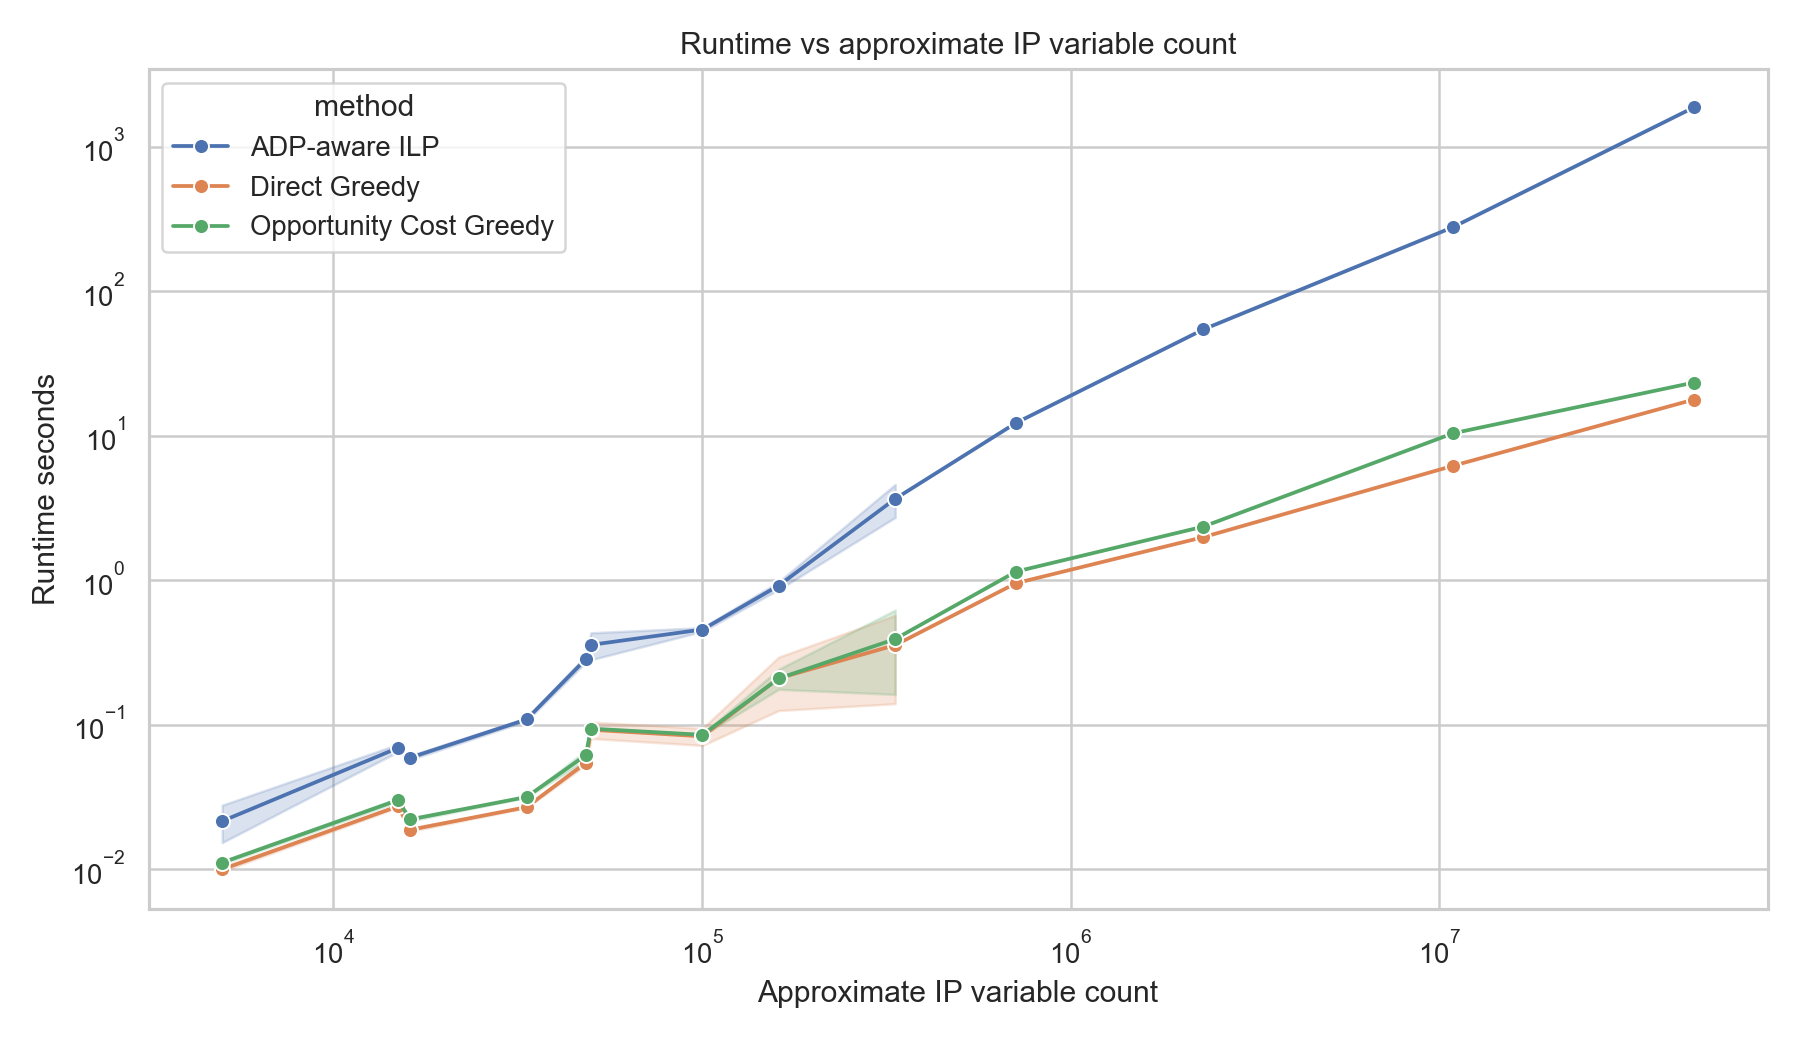
\includegraphics[width=0.70\linewidth]{experiments/synthetic/scaling_summary/runtime_by_variable_count.png}
\caption{Runtime grows sharply for the exact benchmark, while both heuristics remain fast on large synthetic instances.}
\end{figure}

\subsection{Real-data validation}
The 2026 Yahoo and FanGraphs benchmarks are realistic validation cases rather than the main experiment grid. Each dataset has 252 benchmark cases. Table~\ref{tab:real} again shows that Opportunity Cost Greedy has smaller gaps than Direct Greedy.

\begin{table}[H]
\centering
\small
\caption{2026 real-data validation summary.}
\label{tab:real}
\begin{tabular}{llrrr}
\toprule
Dataset & Method & Mean objective & Mean gap & Max gap\\
\midrule
Yahoo 2026 & ADP-aware ILP & 7917.209 & 0.000 & 0.000\\
Yahoo 2026 & Opportunity Cost Greedy & 7767.732 & 149.477 & 255.700\\
Yahoo 2026 & Direct Greedy & 7662.866 & 254.343 & 373.000\\
FanGraphs 2026 & ADP-aware ILP & 14642.927 & 0.000 & 0.000\\
FanGraphs 2026 & Opportunity Cost Greedy & 14320.135 & 322.792 & 508.000\\
FanGraphs 2026 & Direct Greedy & 14097.337 & 545.590 & 644.500\\
\bottomrule
\end{tabular}
\end{table}

\section{Conclusions}
The ADP-aware ILP provides a precise exact benchmark for fantasy baseball draft optimization on manageable instances. Direct Greedy is useful as a simple benchmark heuristic, but it often leaves more value on the table. Opportunity Cost Greedy, our proposed scalable heuristic, captures the value of drafting before a position deteriorates and includes a fallback for tight feasibility. Across synthetic experiments and real-data validation, it consistently improves over Direct Greedy while remaining fast.

The main implication is that exact optimization is valuable for benchmarking and small to medium instances, while a carefully designed heuristic is necessary for large-scale draft planning. Future work could add opponent-specific draft behavior, use calibrated scoring variants as robustness checks, and combine the heuristic with small local ILP subproblems for dynamic in-draft replanning.

\end{document}
